% !TeX program = xelatex
\documentclass[12pt,a4paper]{ctexart}

% ── 页面布局 ──────────────────────────────────────────────
\usepackage[margin=2.5cm]{geometry}

% ── 图表 ──────────────────────────────────────────────────
\usepackage{graphicx}
\usepackage{float}
\usepackage{booktabs}
\usepackage{longtable}
\usepackage{array}

% ── 超链接 ────────────────────────────────────────────────
\usepackage[colorlinks=true,linkcolor=blue,urlcolor=blue]{hyperref}

% ── 标题 ──────────────────────────────────────────────────
\usepackage[font=small,labelfont=bf]{caption}

% ── 数学 ──────────────────────────────────────────────────
\usepackage{amsmath}

\title{\textbf{Visual Lego 计数器}\\[6pt]
       \large 数字图像处理课程项目报告\\[4pt]
       \normalsize AU3304}
\author{}
\date{}

\begin{document}

\maketitle

% ═══════════════════════════════════════════════════════════
\section{引言}
% ═══════════════════════════════════════════════════════════

乐高积木是全球最受欢迎的玩具之一。然而对于乐高零售商而言，人工盘点货架照片中的零件数量既繁琐又容易出错。本项目旨在开发一种自动化方法，从乐高积木堆的俯拍照片中检测、分类并计数单个积木零件。

测试数据集包含 10 张图像，分为三个难度等级：

\begin{itemize}
    \item \textbf{简单（图1--4）：} 主要为 Brick 和 Plate，无遮挡。
    \item \textbf{中等（图5--7）：} 零件种类更多，排列更复杂。
    \item \textbf{困难（图8--10）：} 存在遮挡和多样化的摆放姿态。
\end{itemize}

相同形状但不同颜色的零件合并计数，不同尺寸的零件分别计数。根据课程提供的零件目录，测试图像中可能出现 18 种不同类型的乐高零件，涵盖标准砖块、平板、轮胎、轮毂、窗框等。

% ═══════════════════════════════════════════════════════════
\section{方法}
% ═══════════════════════════════════════════════════════════

\subsection{总体流程}

本方案的检测流程分为三个阶段：

\begin{enumerate}
    \item \textbf{合成训练数据生成} —— 利用零件的多视角模板图片，通过图像合成和随机增强，生成带标注的训练数据集。
    \item \textbf{YOLOv8 模型训练} —— 在合成数据集上微调 YOLOv8 nano 检测模型。
    \item \textbf{推理} —— 将训练好的模型应用于测试图像，检测并分类单个积木零件。
\end{enumerate}

\subsection{合成训练数据生成}

由于缺乏人工标注的训练数据，本方案通过将模板图像合成到真实背景上来程序化地生成训练数据。

\textbf{模板图像}：从 LDraw.org 和 BrickLink.com 收集了全部 18 种乐高零件的多视角模板图像（俯视、仰视、侧视、等轴测视图，共 79 张）。训练数据生成仅使用俯视图（21 张），因为测试照片均为俯拍。

每张合成图像的\textbf{生成步骤}如下：

\begin{enumerate}
    \item 从原始测试图像中随机截取一块作为背景。
    \item 从不同类别中随机选取 3--15 个零件模板。
    \item 对每个零件应用随机增强：
    \begin{itemize}
        \item 旋转 $\pm 30^\circ$
        \item 缩放 $0.6\times$--$1.2\times$
        \item 亮度 $\pm 15\%$，对比度 $\pm 15\%$
        \item HSV 色调偏移，模拟不同颜色
    \end{itemize}
    \item 通过阈值分割创建零件蒙版（模板背景为白色），使用 alpha 混合将零件叠加到画布上，并添加投影阴影。
    \item 对合成图像应用与测试图像相同的预处理流程（多尺度阴影去除 + CLAHE 对比度增强）。
    \item 输出 $640\times640$ 的合成图像及 YOLO 格式的边界框标签。
\end{enumerate}

最终生成 \textbf{600 张}合成图像（468 张训练，132 张验证），共计约 5,300 个标注框，覆盖全部 18 个类别。

\subsection{模型训练}

使用 \textbf{YOLOv8 nano} 模型（301 万参数），从 COCO 预训练权重开始进行微调。训练在 CPU 上完成。

\begin{table}[H]
    \centering
    \caption{训练配置}
    \label{tab:training}
    \begin{tabular}{ll}
        \toprule
        \textbf{参数} & \textbf{取值} \\
        \midrule
        输入尺寸   & $640\times640$ \\
        批次大小   & 8 \\
        训练轮数   & 50 \\
        优化器     & AdamW（学习率 $4.55\times10^{-4}$）\\
        设备       & CPU（AMD Ryzen 7 5800H）\\
        训练耗时   & 1.7 小时 \\
        数据增强   & Mosaic、随机水平翻转、HSV 抖动、缩放、平移、RandAugment、随机擦除 \\
        \bottomrule
    \end{tabular}
\end{table}

合成验证集上的训练结果为：\textbf{mAP@50 = 0.899}，\textbf{mAP@50--95 = 0.781}，精确率 0.935，召回率 0.840。

\begin{figure}[H]
    \centering
    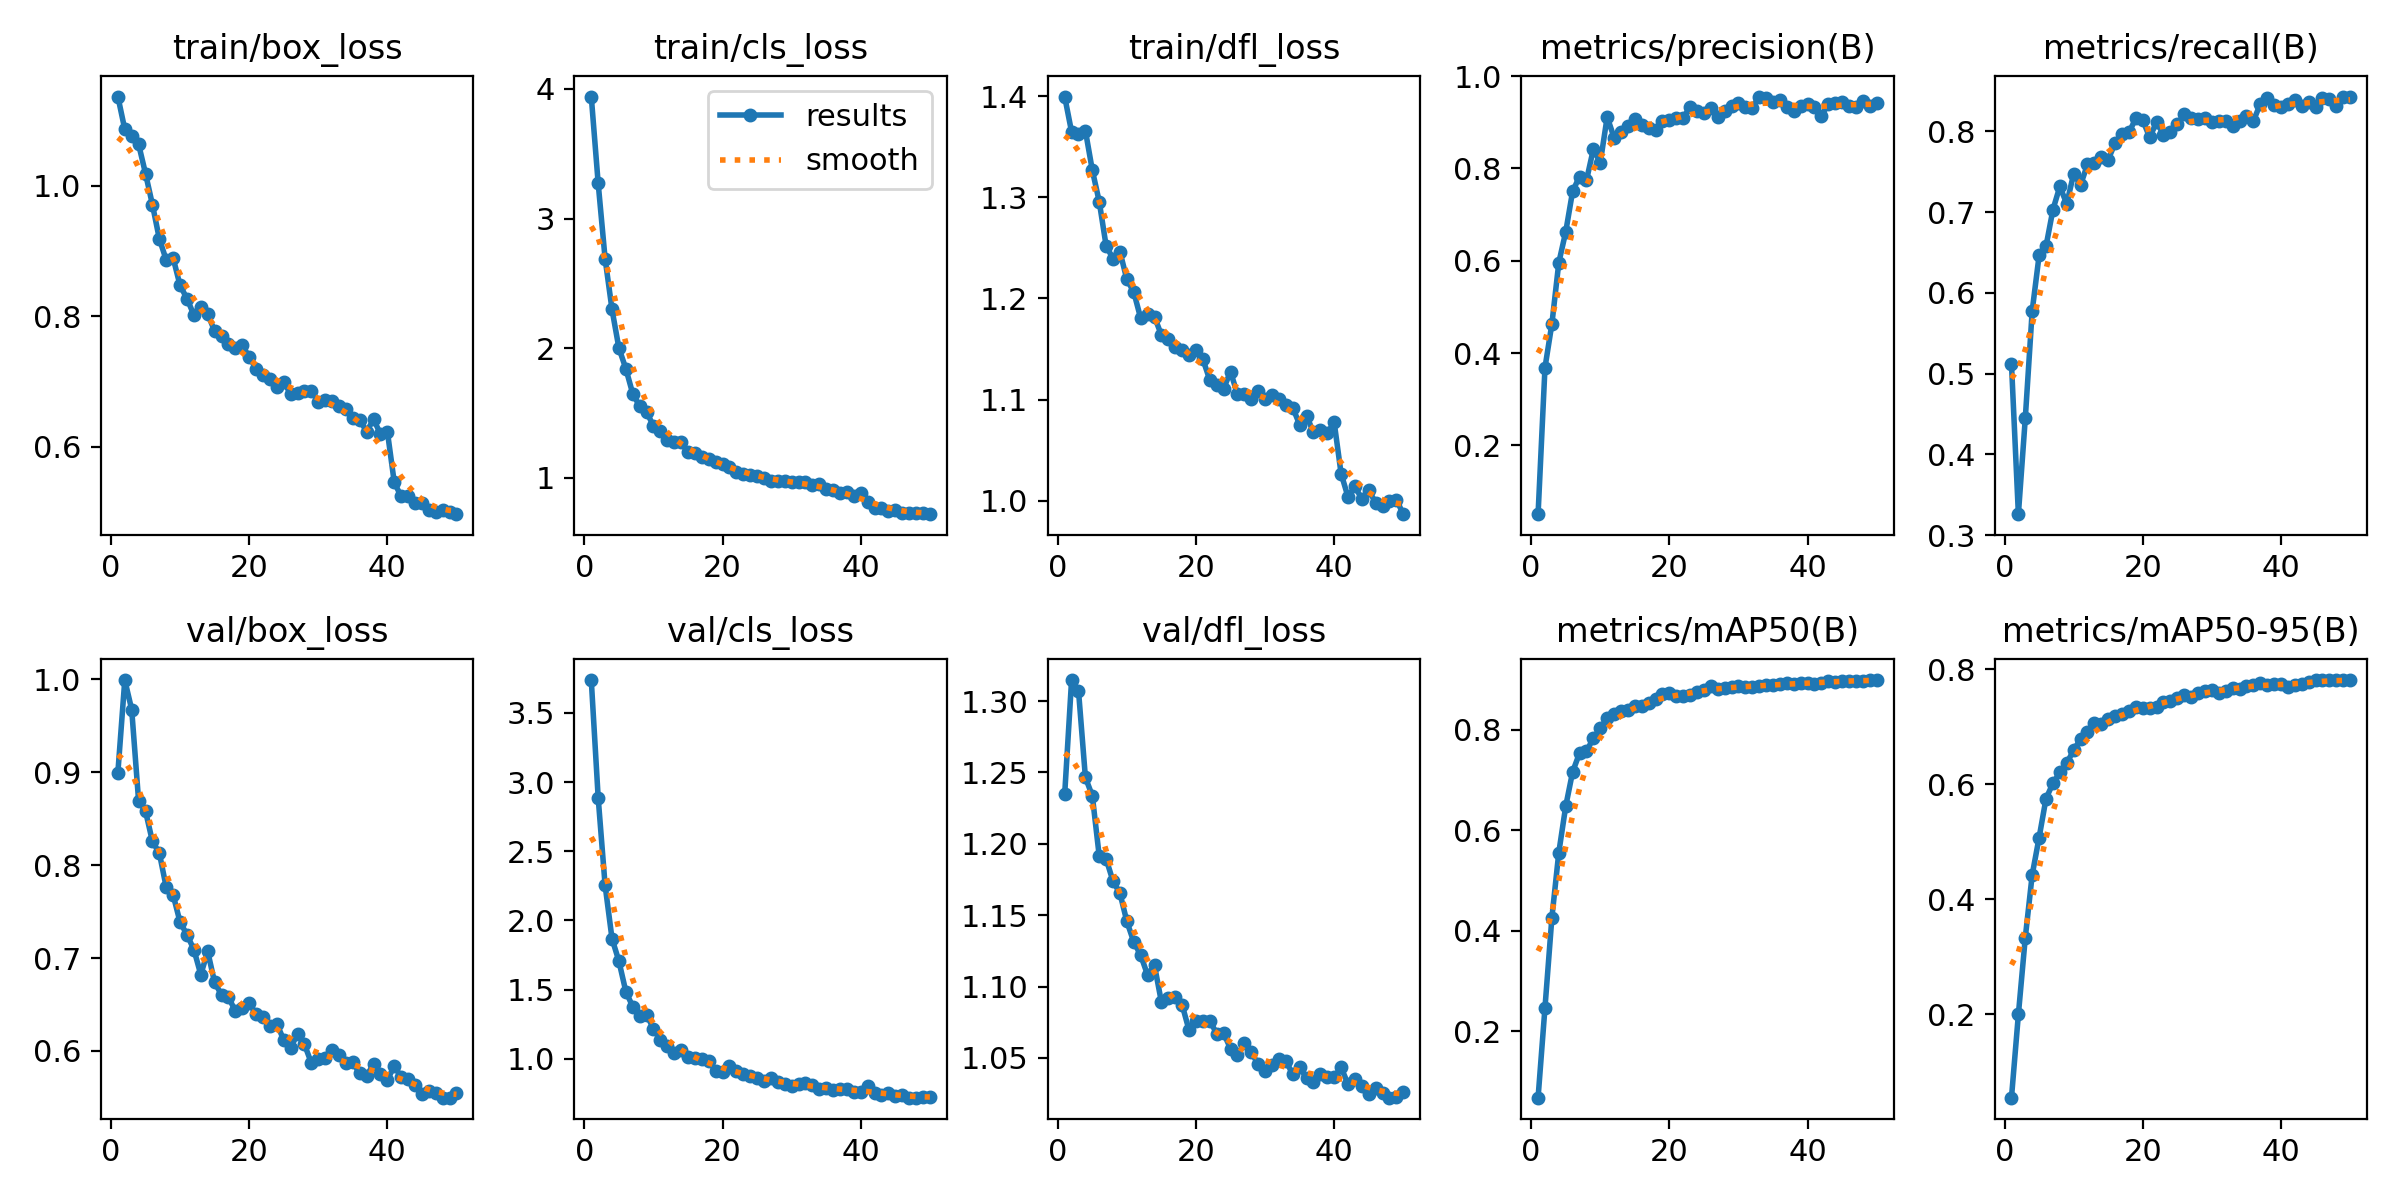
\includegraphics[width=\textwidth]{figures/training_curves.png}
    \caption{训练过程曲线。从上到下依次为：边界框损失、分类损失、DFL 损失；精确率、召回率、mAP@50、mAP@50--95（验证集）。模型在约 30 轮后趋于收敛。}
    \label{fig:curves}
\end{figure}

\begin{figure}[H]
    \centering
    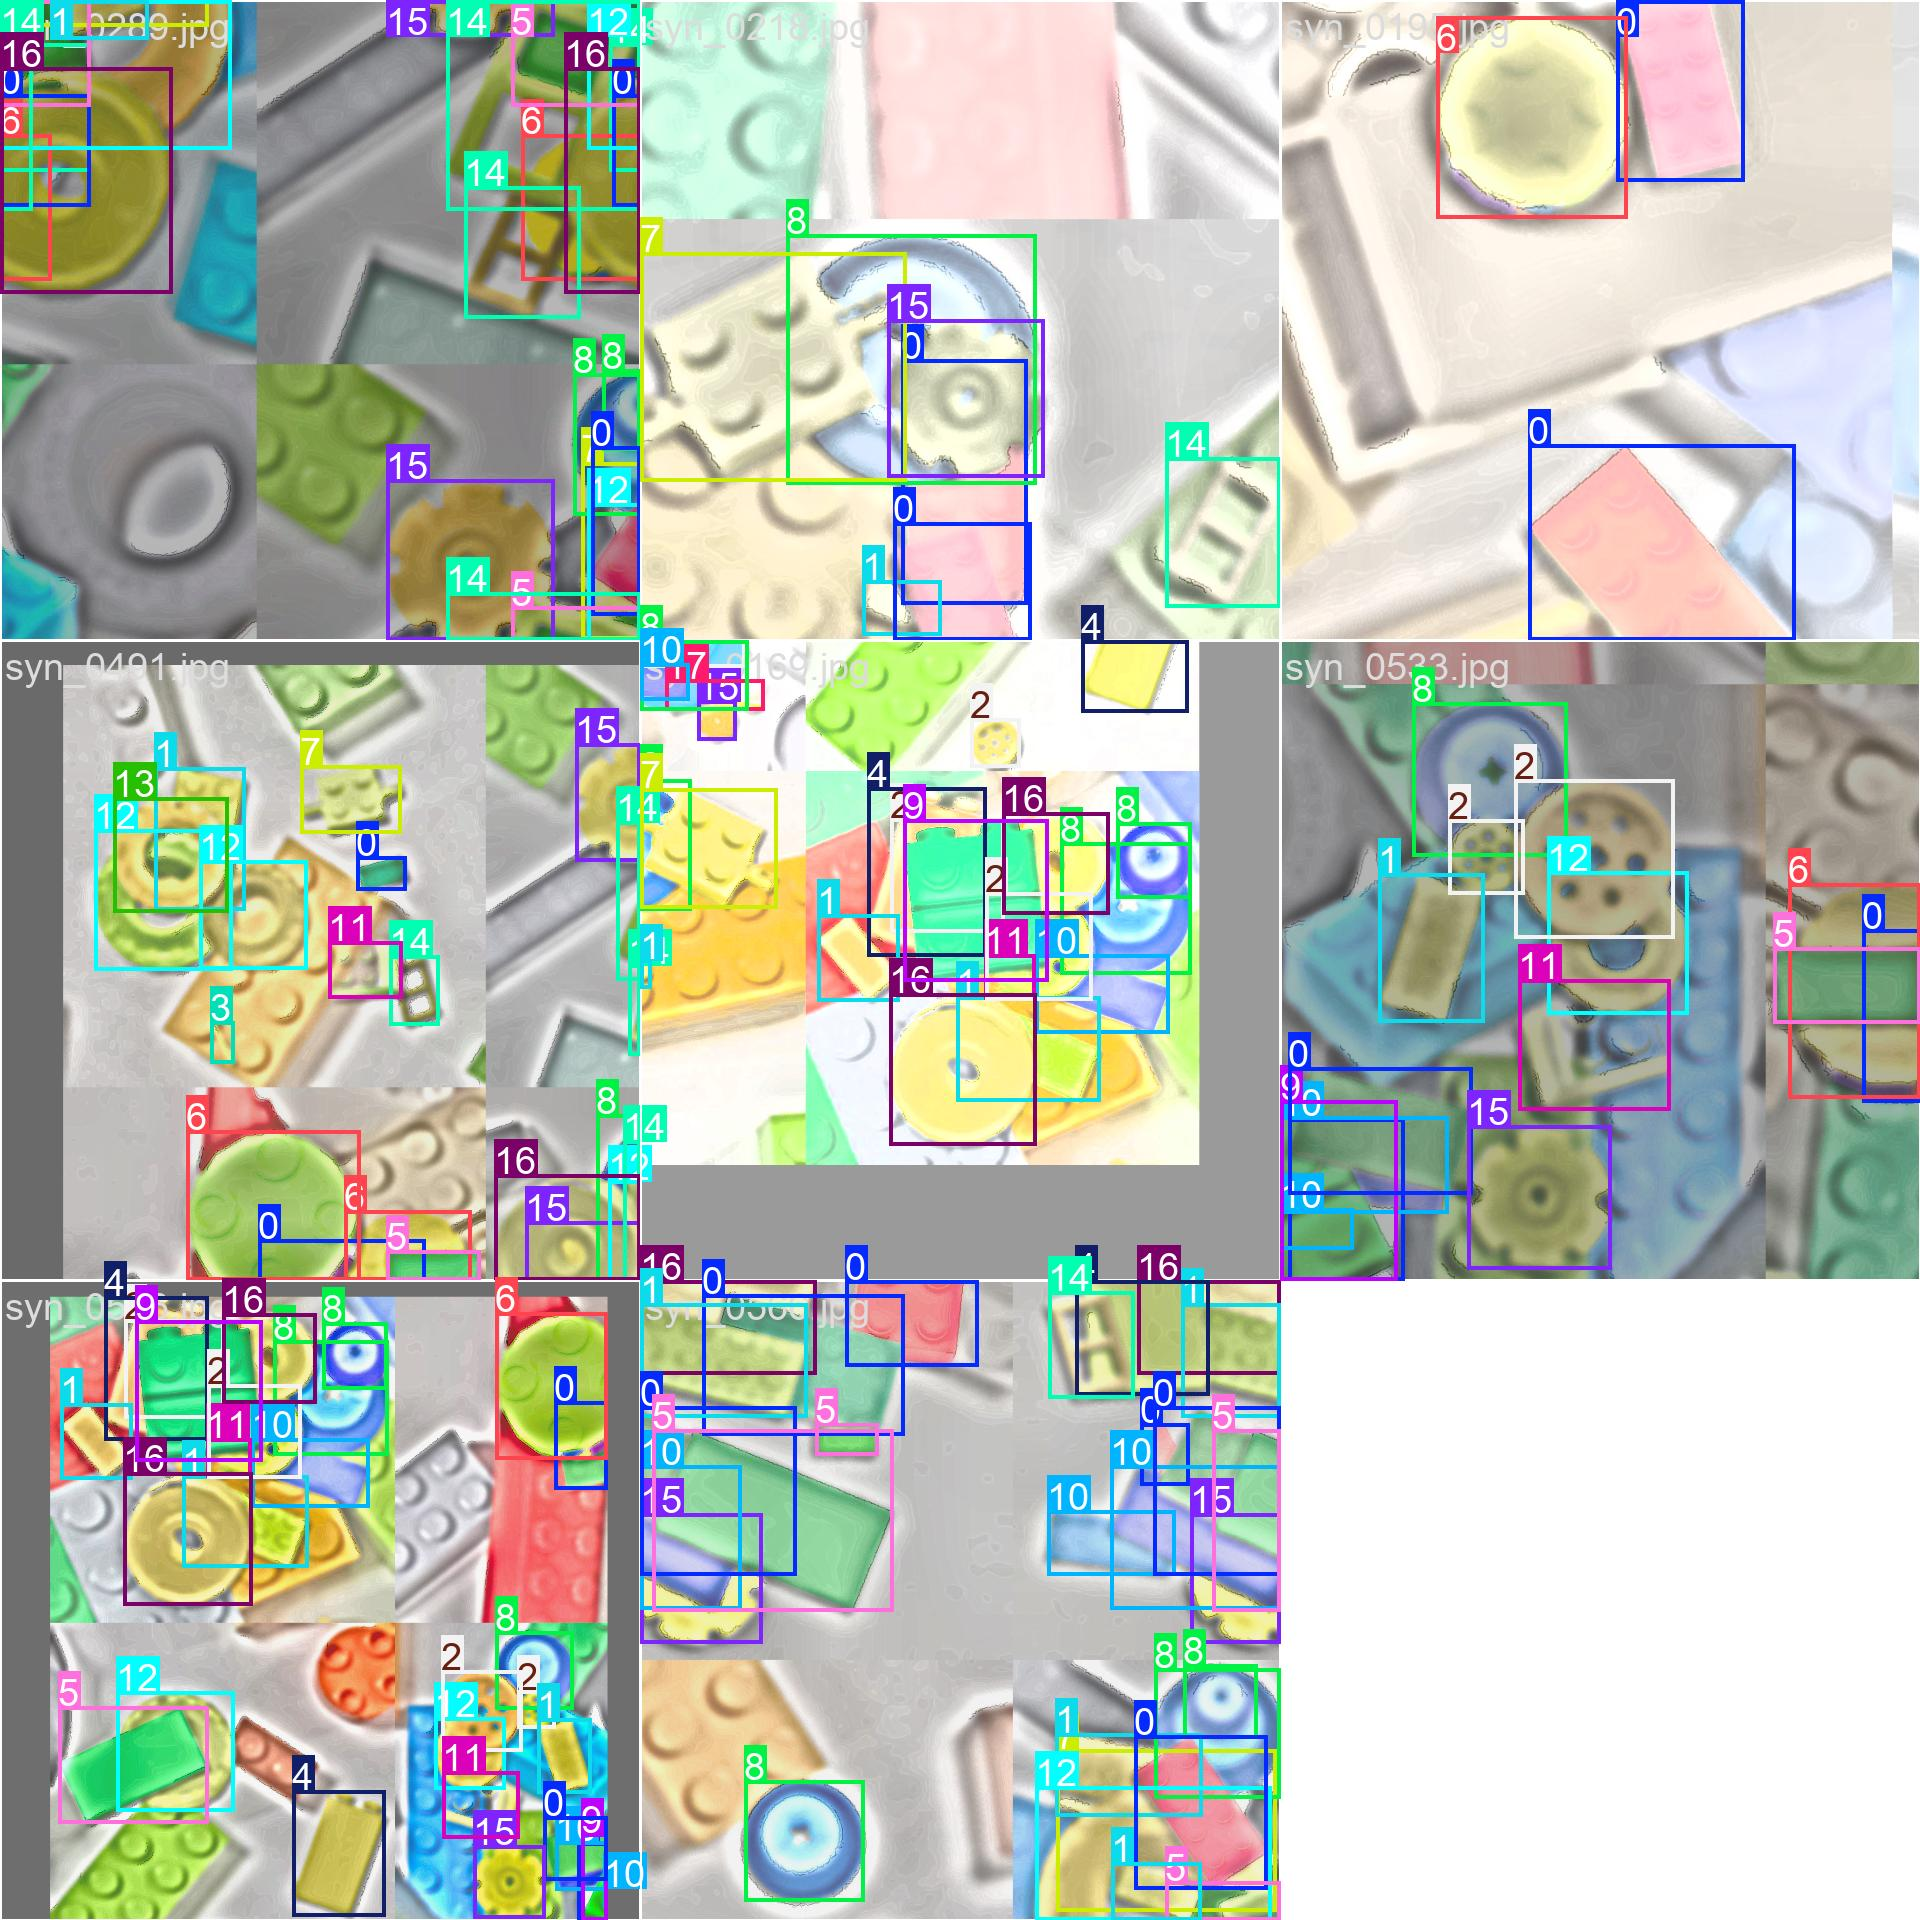
\includegraphics[width=0.7\textwidth]{figures/train_batch.jpg}
    \caption{合成训练数据样本。零件被随机粘贴到真实背景上，附带旋转、缩放、颜色增强和投影阴影。}
    \label{fig:trainbatch}
\end{figure}

\subsection{推理}

将训练好的模型应用于全部 10 张测试图像，置信度阈值设为 0.3。模型对每张图像输出每个检测到的零件的边界框、类别标签和置信度。

% ═══════════════════════════════════════════════════════════
\section{实验结果}
% ═══════════════════════════════════════════════════════════

\subsection{总览}

在全部 10 张图像中共检出 \textbf{241} 个零件，覆盖 \textbf{18 个类别中的 16 个}。未检出的两个类别为：

\begin{itemize}
    \item Wheel Rim 20x30 with 6 Dual Spokes and External Ribs
    \item Plate 2x2 with 2 Studs on the side
\end{itemize}

这两个类别在训练数据中均仅有一张模板图像，且从俯视角度观察时易与其他相似零件混淆。

\begin{figure}[H]
    \centering
    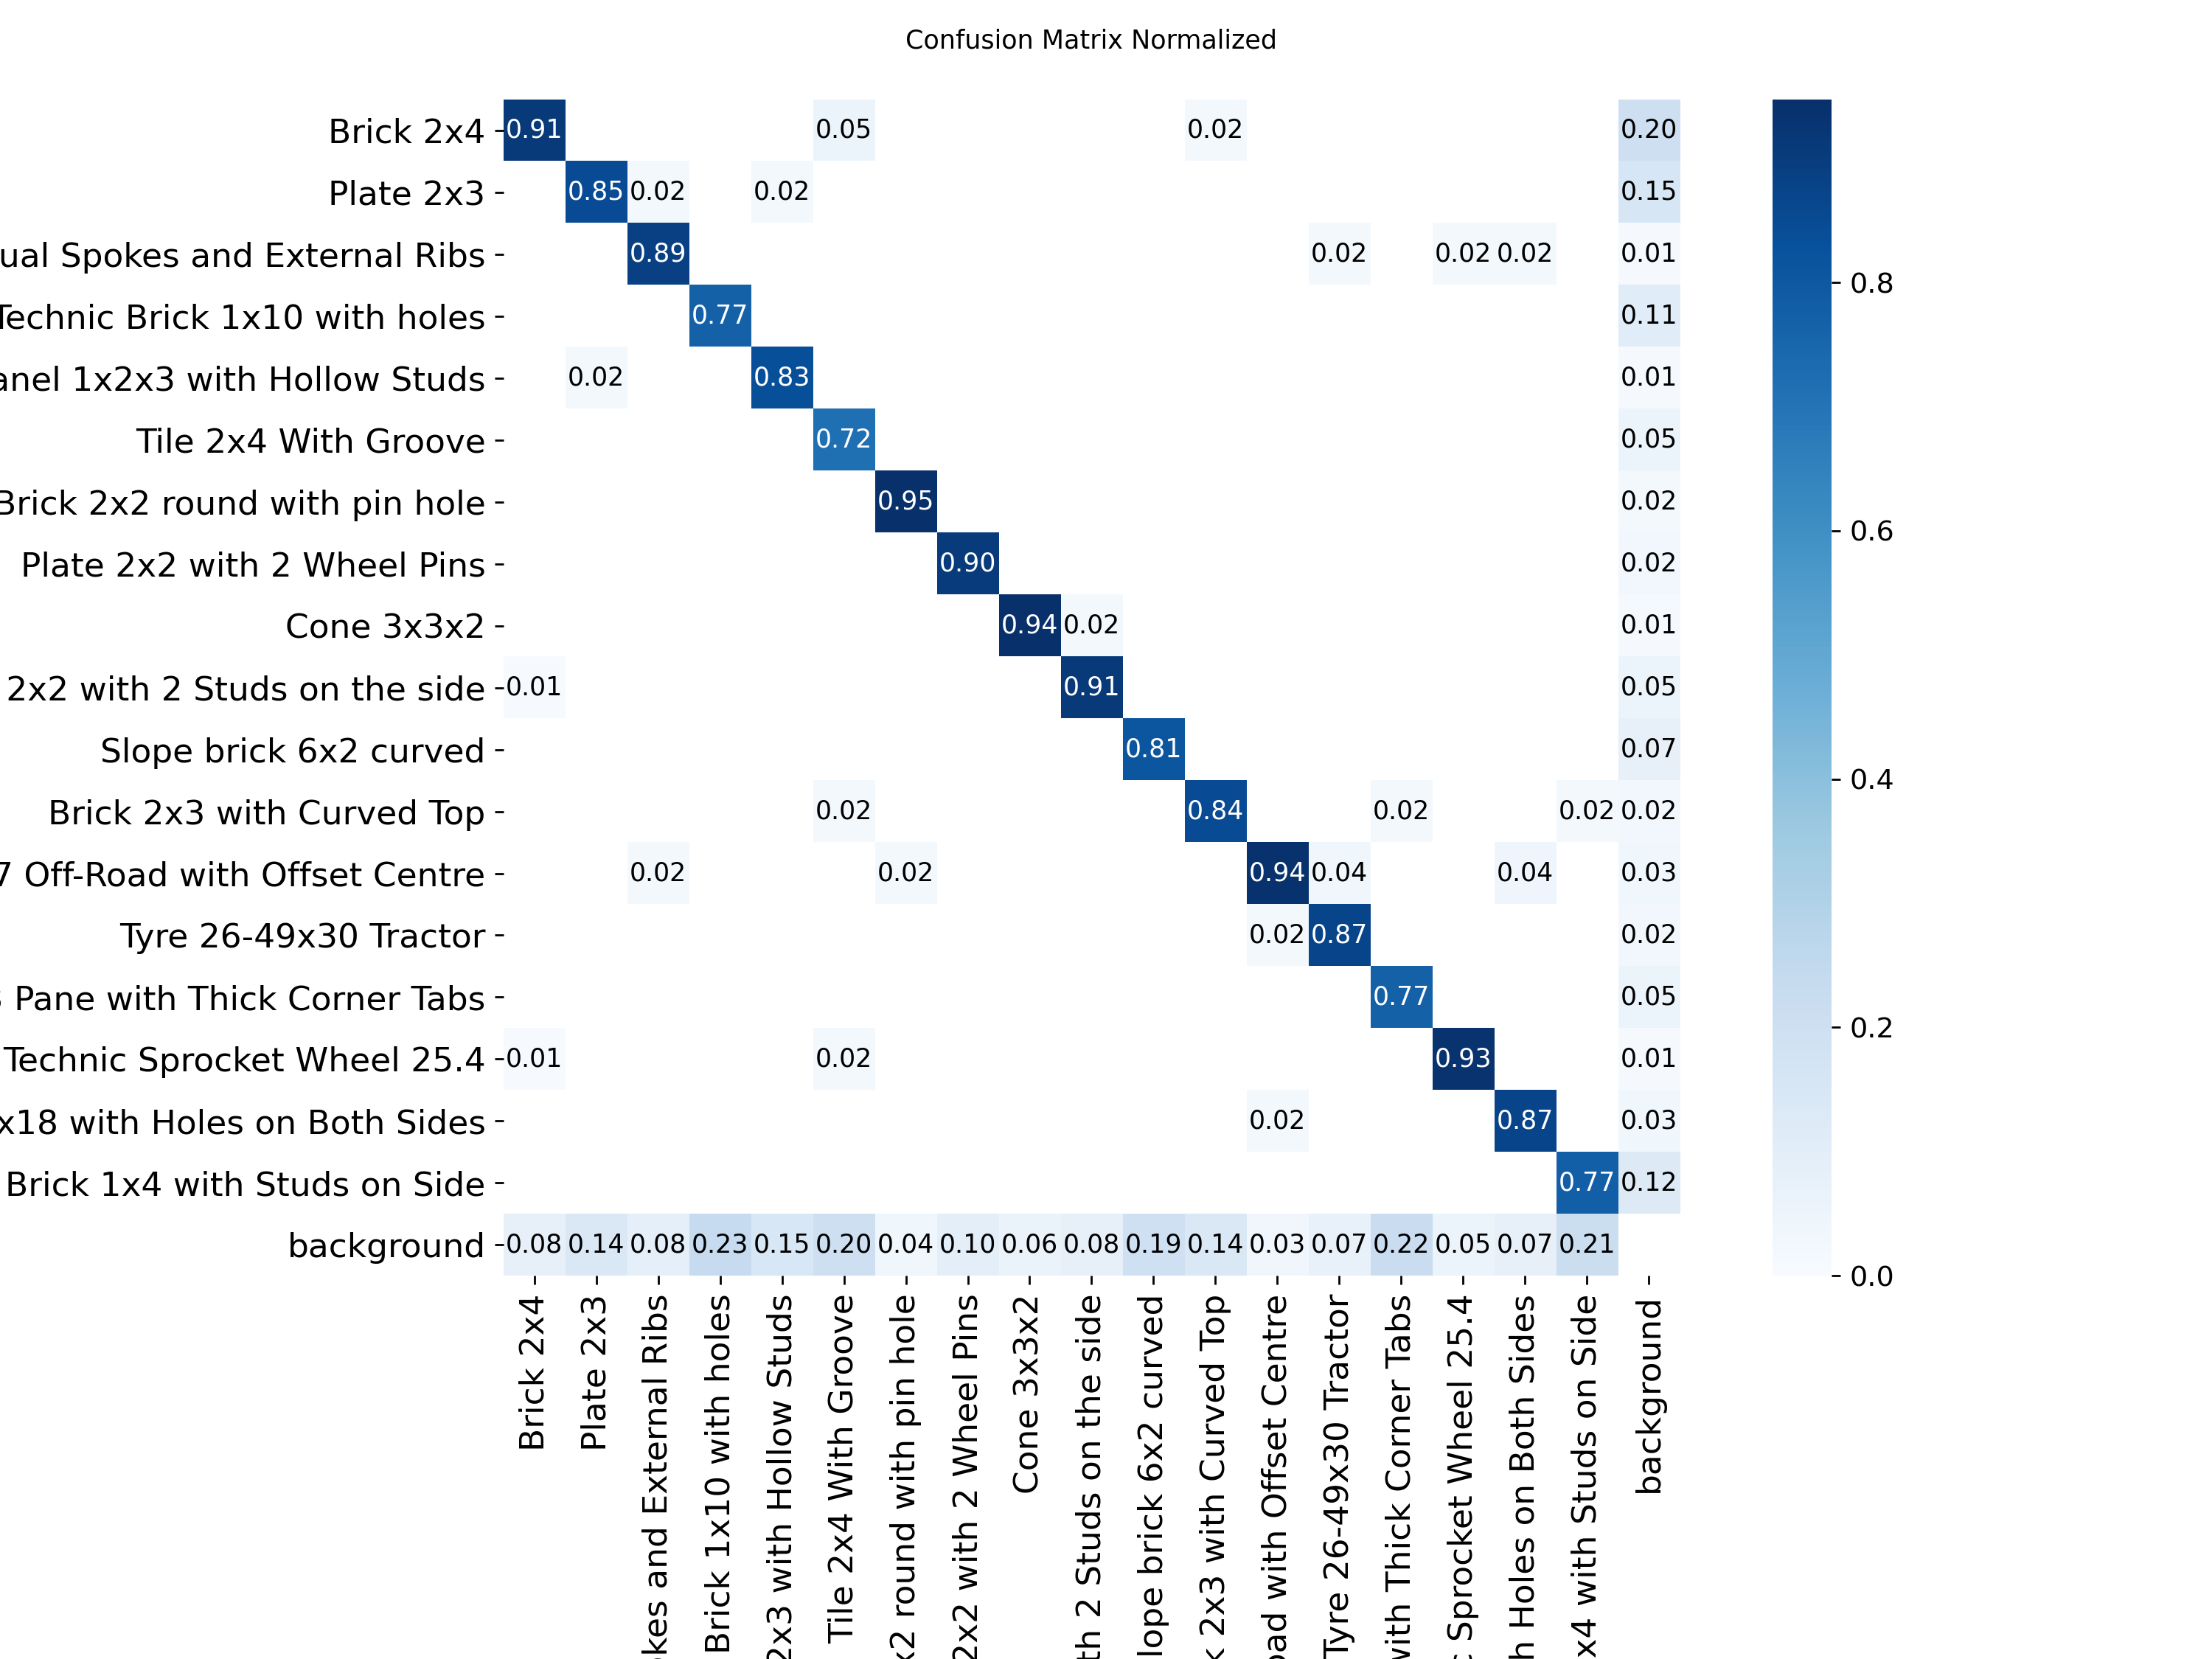
\includegraphics[width=0.85\textwidth]{figures/confusion_matrix.png}
    \caption{归一化混淆矩阵（合成验证集）。对角线越亮表示该类别分类越准确。大部分类别沿对角线集中，少数类别（如类别 10 与 11）存在一定混淆。}
    \label{fig:confusion}
\end{figure}

\begin{figure}[H]
    \centering
    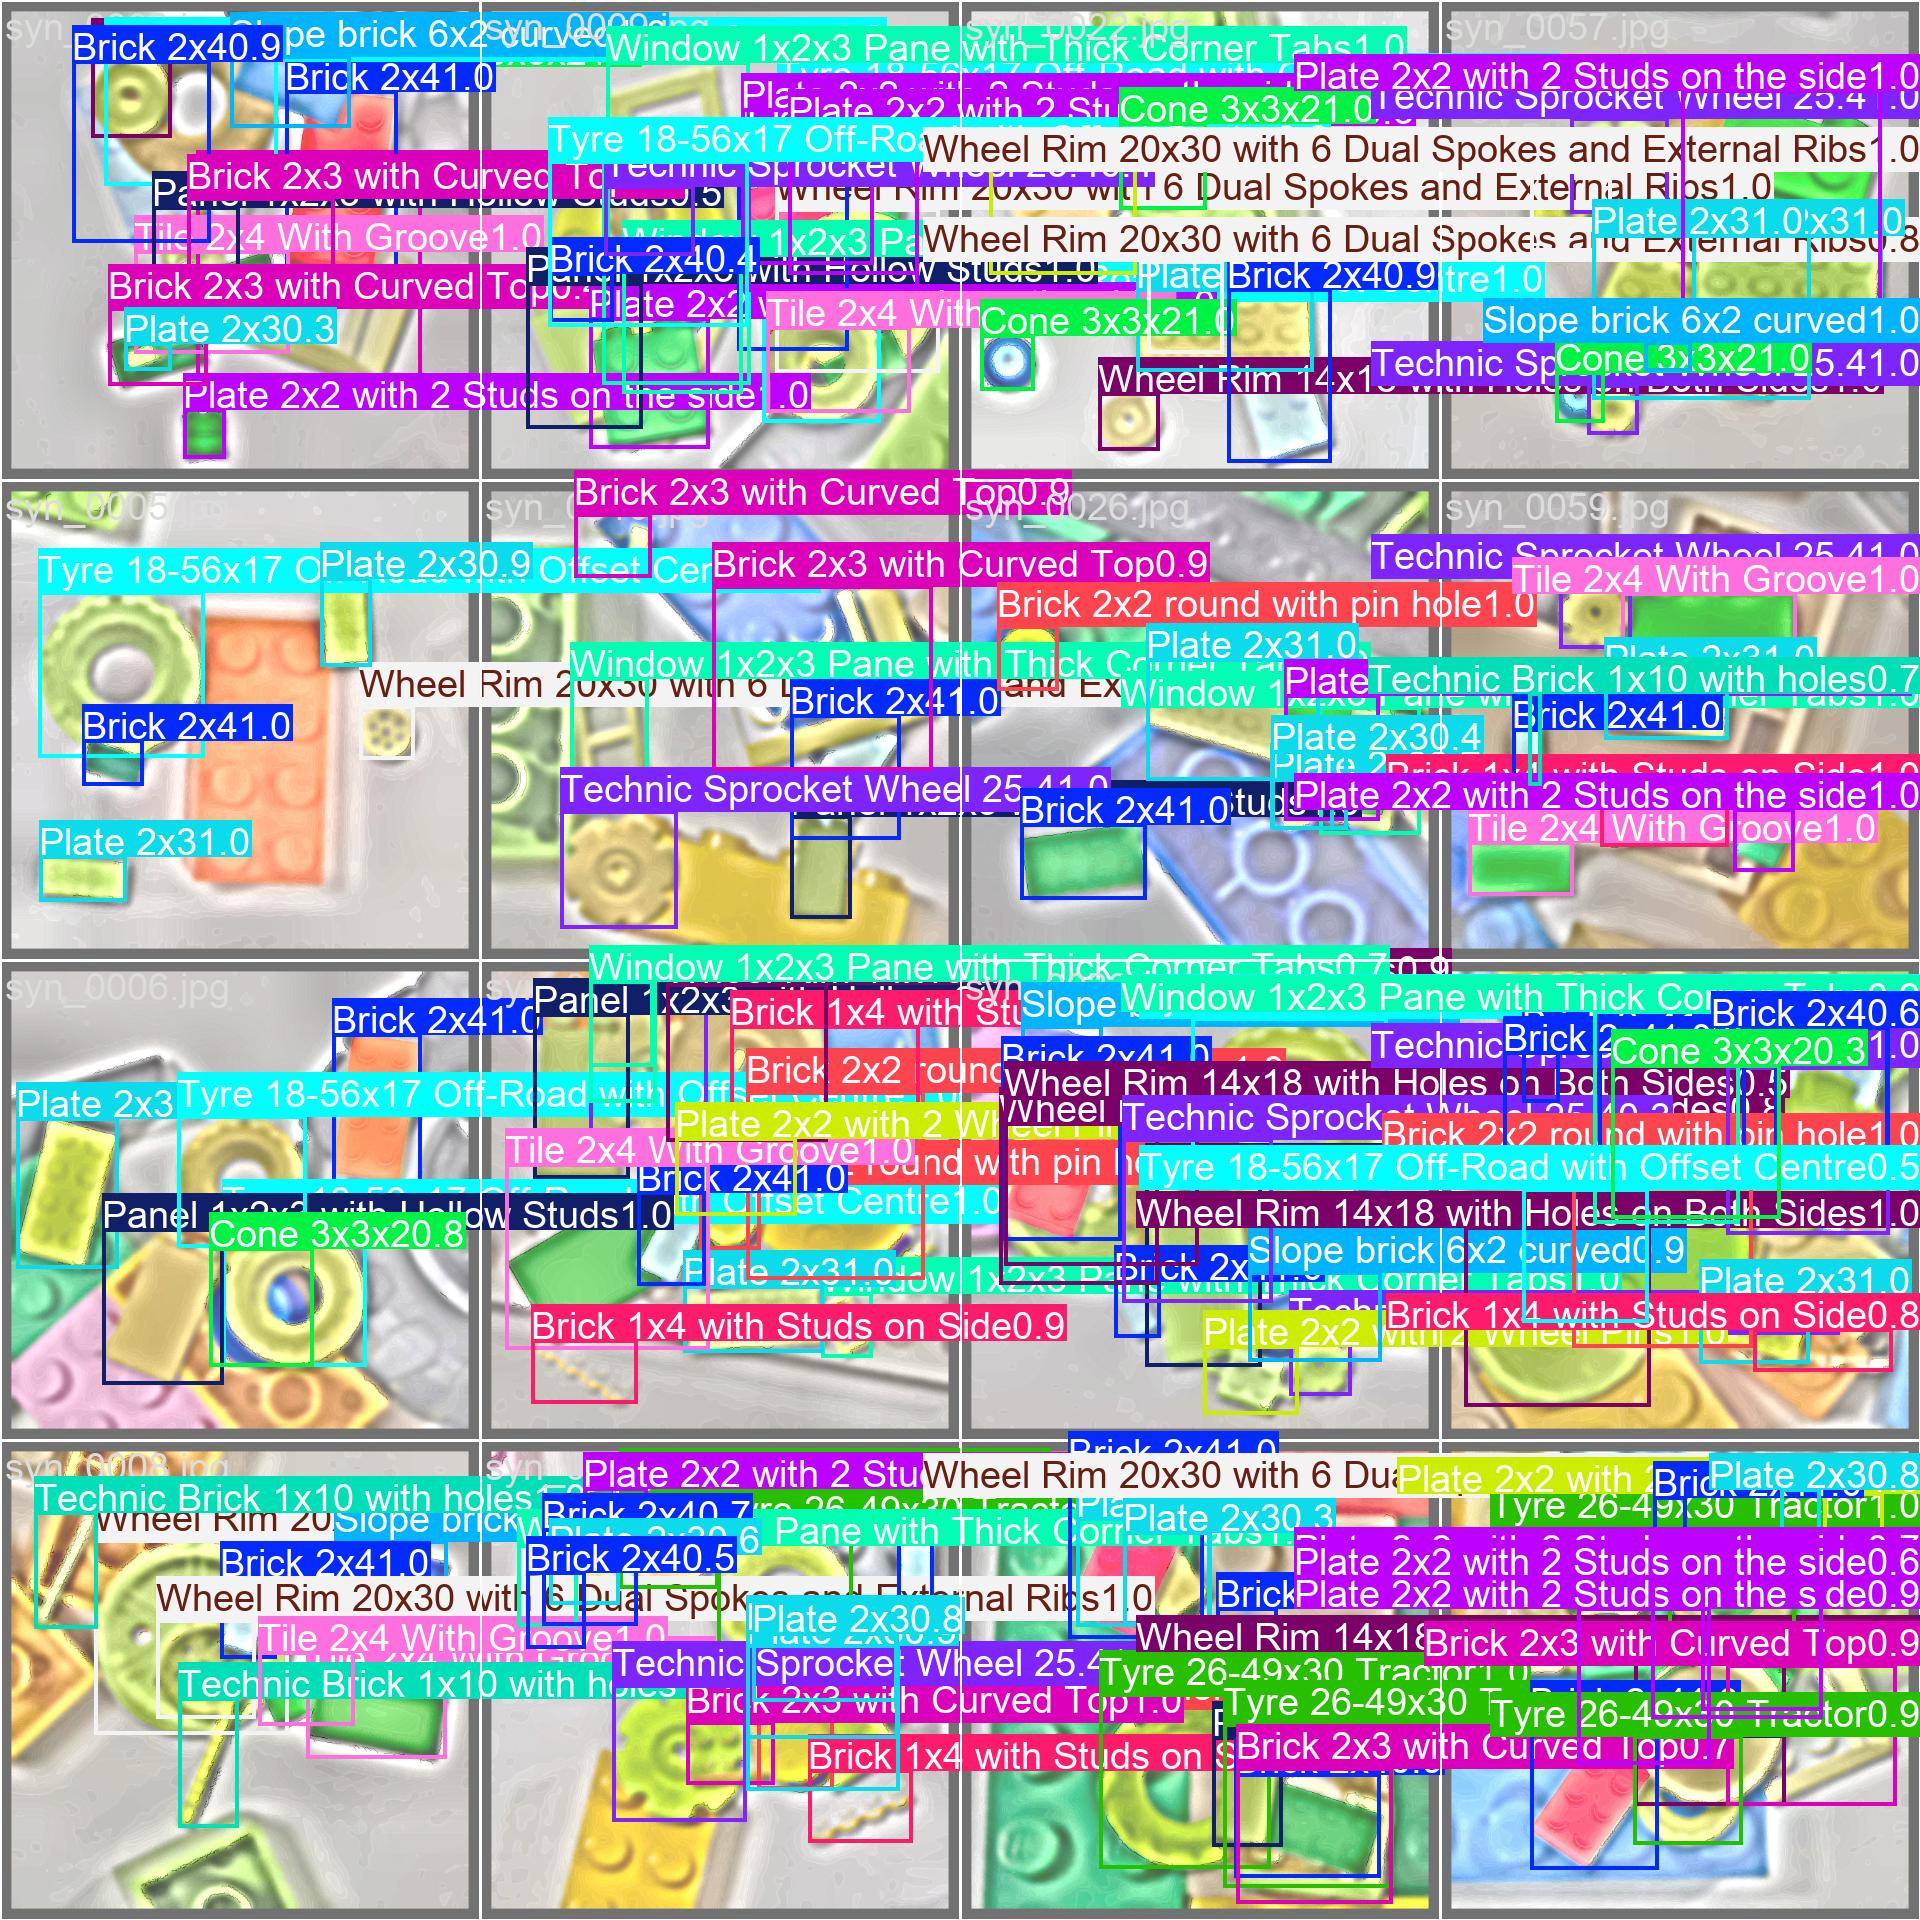
\includegraphics[width=0.75\textwidth]{figures/val_pred.jpg}
    \caption{验证集预测样例。绿色框为模型预测结果，标签显示类别名称与置信度。}
    \label{fig:valpred}
\end{figure}

\subsection{逐图结果}

\begin{table}[H]
    \centering
    \caption{各图像检测结果汇总。S=简单，M=中等，H=困难。}
    \label{tab:perimage}
    \small
    \begin{tabular}{cccl}
        \toprule
        \textbf{图像} & \textbf{难度} & \textbf{检出数} & \textbf{类别组成（数量 × 零件名）} \\
        \midrule
        1  & S & 17 & Brick 2x4 (10), Plate 2x3 (6), Window (1) \\
        2  & S & \textbf{2}  & Brick 2x4 (2) \\
        3  & S & 23 & Brick 2x4 (13), Plate 2x3 (9), Technic 1x10 (1) \\
        4  & S & 34 & Brick 2x4 (17), Plate 2x3 (13), Technic 1x10 (3), Slope 6x2 (1) \\
        \addlinespace
        5  & M & 17 & Brick 2x4 (6), Plate 2x3 (6), Curved Top (2), Panel (1), Tile (1), Window (1) \\
        6  & M & 35 & Brick 2x4 (13), Plate 2x3 (12), Slope 6x2 (4), 及其它 6 类 \\
        7  & M & 28 & Plate 2x3 (11), Brick 2x4 (10), 及其它 7 类 \\
        \addlinespace
        8  & H & 17 & Brick 2x4 (4), Slope 6x2 (4), Plate 2x3 (3), 及其它 4 类 \\
        9  & H & 27 & Brick 2x4 (9), Plate 2x3 (6), Slope 6x2 (4), 及其它 7 类 \\
        10 & H & 41 & Brick 2x4 (21), Plate 2x3 (10), Slope 6x2 (3), 及其它 5 类 \\
        \bottomrule
    \end{tabular}
\end{table}

\subsection{类别分布}

\begin{table}[H]
    \centering
    \caption{各类别检出数量汇总}
    \label{tab:classes}
    \begin{tabular}{lrlr}
        \toprule
        \textbf{类别} & \textbf{数量} & \textbf{类别} & \textbf{数量} \\
        \midrule
        Brick 2x4                    & 105 & Plate 2x3                      & 76 \\
        Slope brick 6x2 curved       & 17  & Technic Brick 1x10 with holes   & 9  \\
        Window 1x2x3 Pane            & 5   & Brick 2x3 with Curved Top       & 5  \\
        Tyre 26-49x30 Tractor        & 5   & Plate 2x2 with 2 Wheel Pins     & 5  \\
        Panel 1x2x3 Hollow Studs     & 3   & Cone 3x3x2                      & 3  \\
        Tile 2x4 With Groove         & 2   & Technic Sprocket Wheel 25.4     & 2  \\
        Brick 1x4 with Studs on Side & 1   & Tyre 18-56x17 Off-Road          & 1  \\
        Wheel Rim 14x18              & 1   & Brick 2x2 round with pin hole   & 1  \\
        \bottomrule
    \end{tabular}
\end{table}

Brick 2x4 和 Plate 2x3 合计占总检出量的 75\%（181/241），与它们在测试图像中的实际分布一致。

\subsection{按难度分析}

\begin{table}[H]
    \centering
    \caption{各难度级别统计}
    \label{tab:difficulty}
    \begin{tabular}{lccc}
        \toprule
        \textbf{难度} & \textbf{图像数} & \textbf{检出总数} & \textbf{检出类别数} \\
        \midrule
        简单（1--4）  & 4  & 76  & 5  \\
        中等（5--7）  & 3  & 80  & 14 \\
        困难（8--10） & 3  & 85  & 12 \\
        \bottomrule
    \end{tabular}
\end{table}

中等难度的检出类别数最高（14 类），简单难度最少（5 类），这与图像中实际出现的零件种类一致。困难难度检出 12 类，比中等略少，原因是遮挡导致部分零件难以识别。

\subsection{检测结果展示}

\begin{figure}[H]
    \centering
    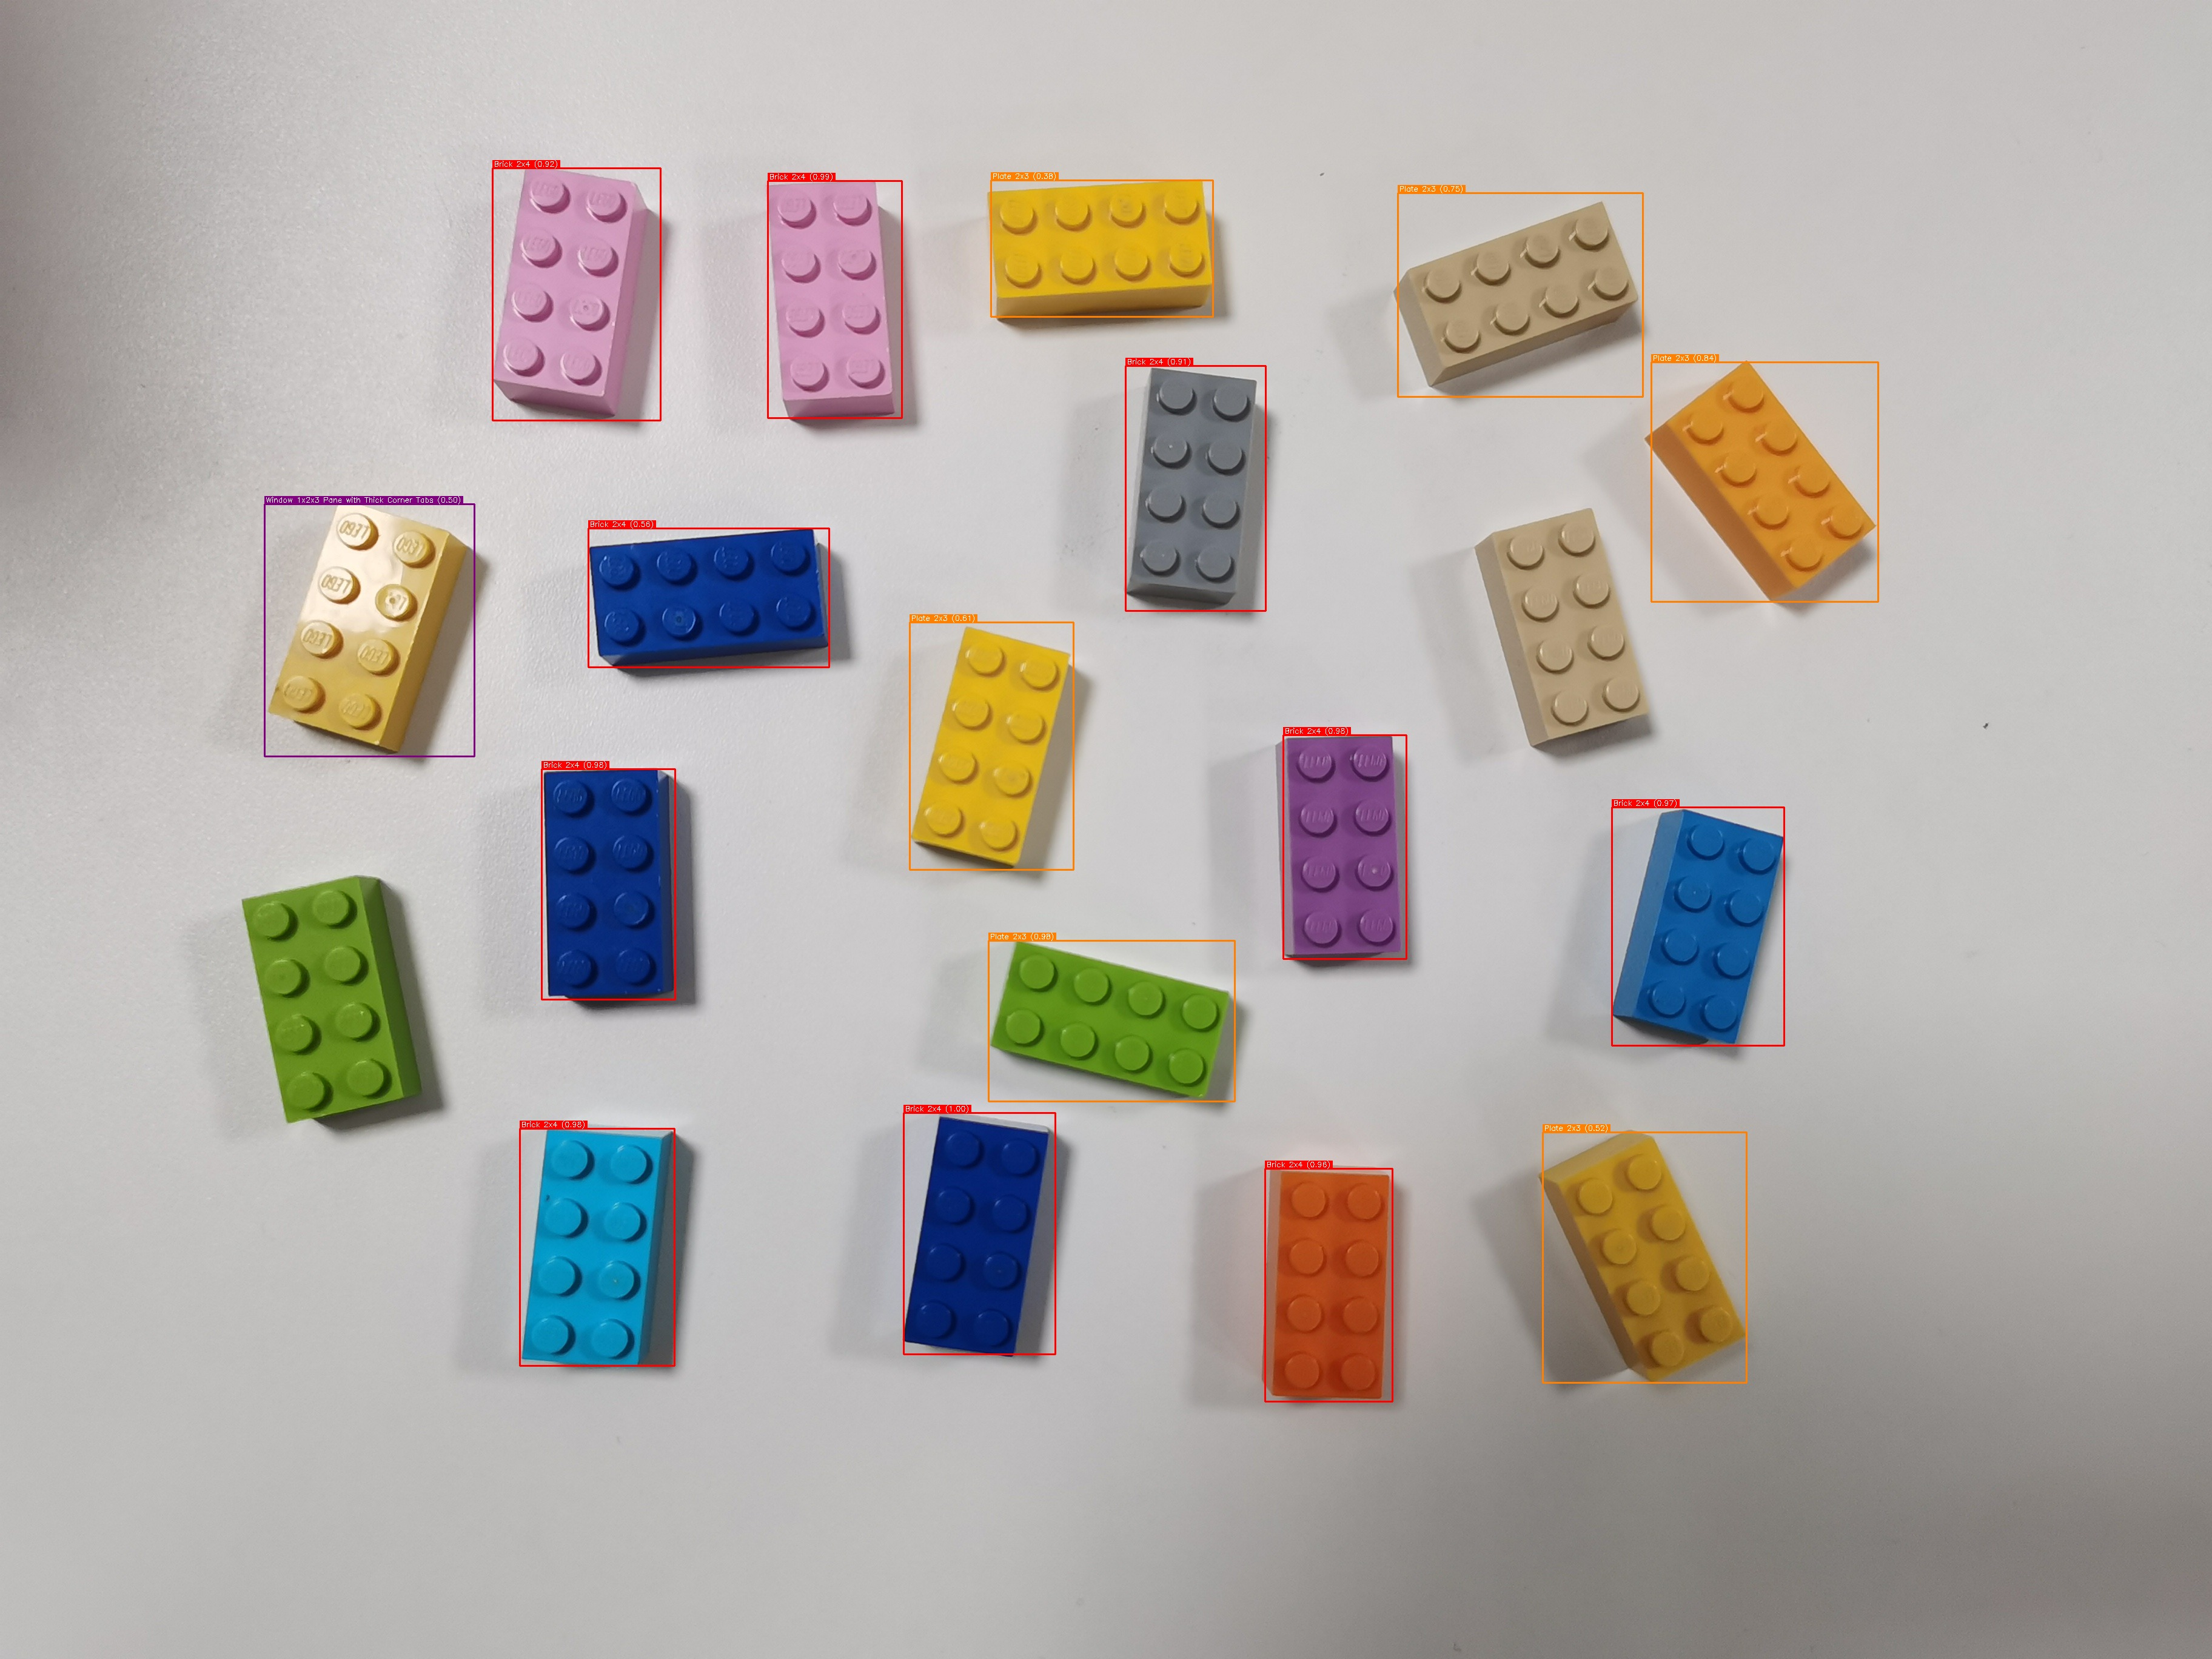
\includegraphics[width=\textwidth]{figures/detect_simple.jpg}
    \caption{简单难度代表（图 1）。检出 17 个零件，3 个类别：Brick 2x4 (10)、Plate 2x3 (6)、Window Pane (1)。零件排列稀疏、无遮挡，检测效果良好。}
    \label{fig:det_simple}
\end{figure}

\begin{figure}[H]
    \centering
    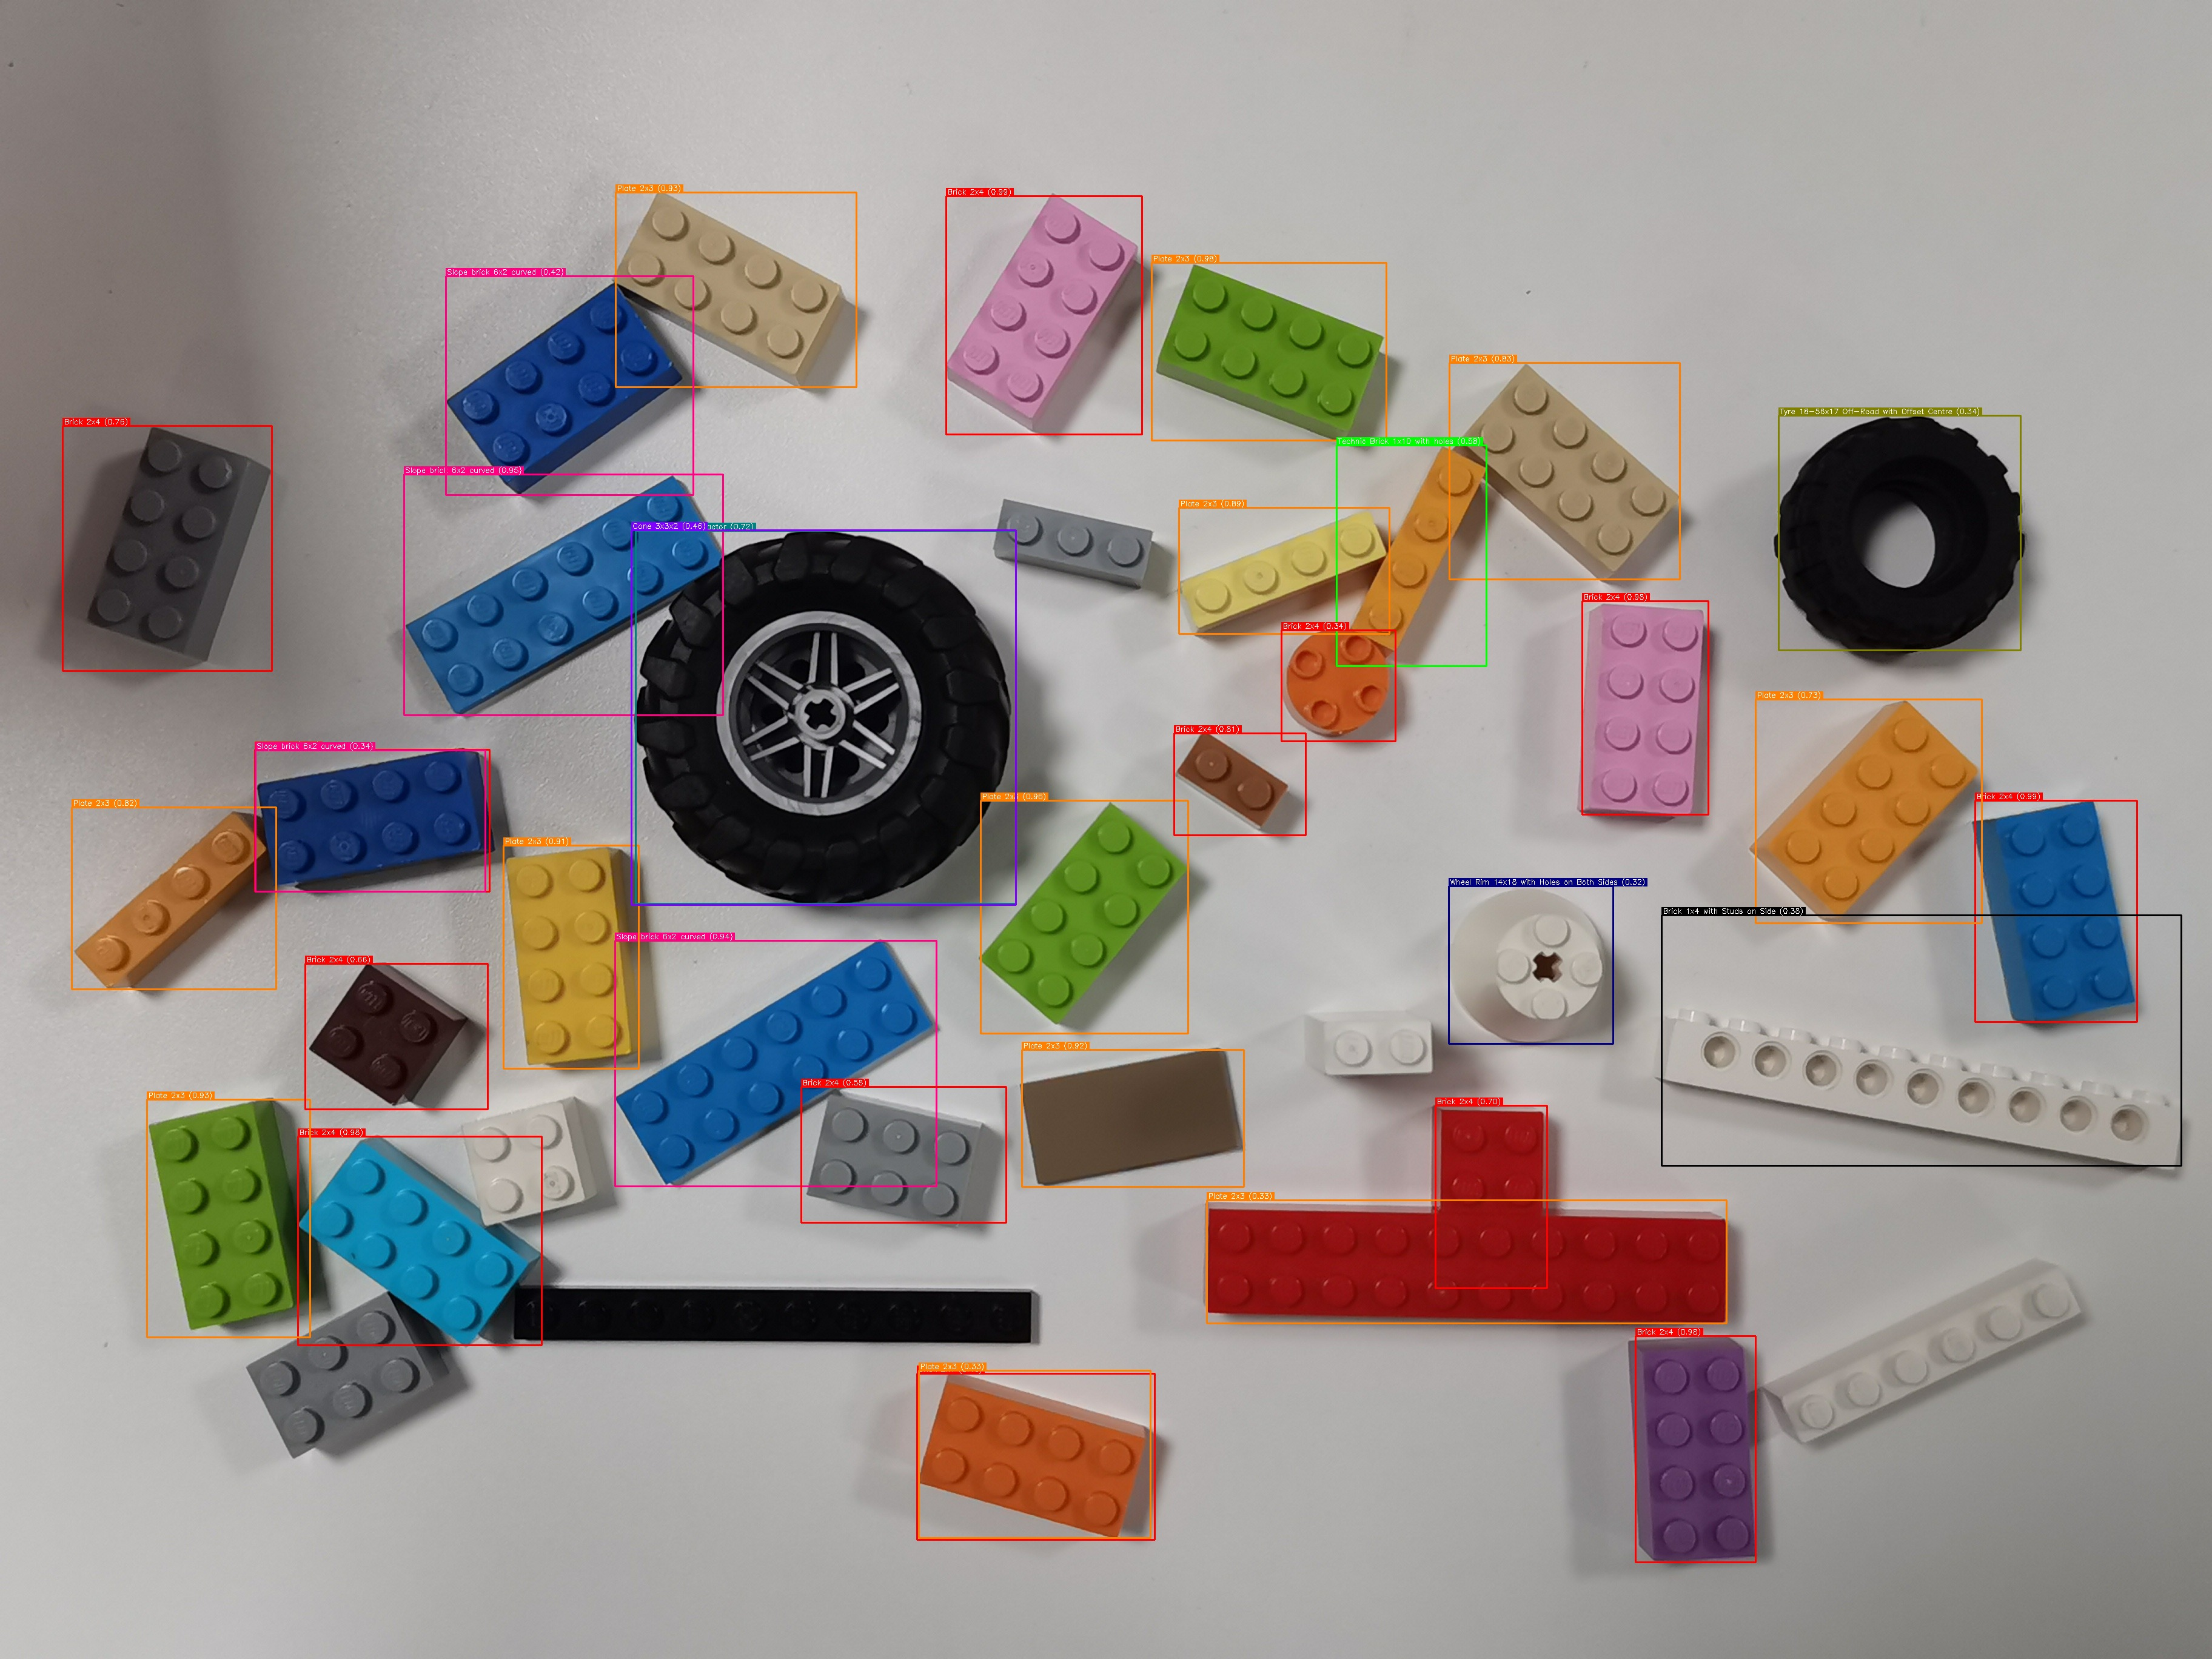
\includegraphics[width=\textwidth]{figures/detect_medium.jpg}
    \caption{中等难度代表（图 6）。检出 35 个零件，9 个类别。Slope 6x2、Tyre、Cone 等多样零件均被检出，验证了合成训练数据的泛化能力。}
    \label{fig:det_medium}
\end{figure}

\begin{figure}[H]
    \centering
    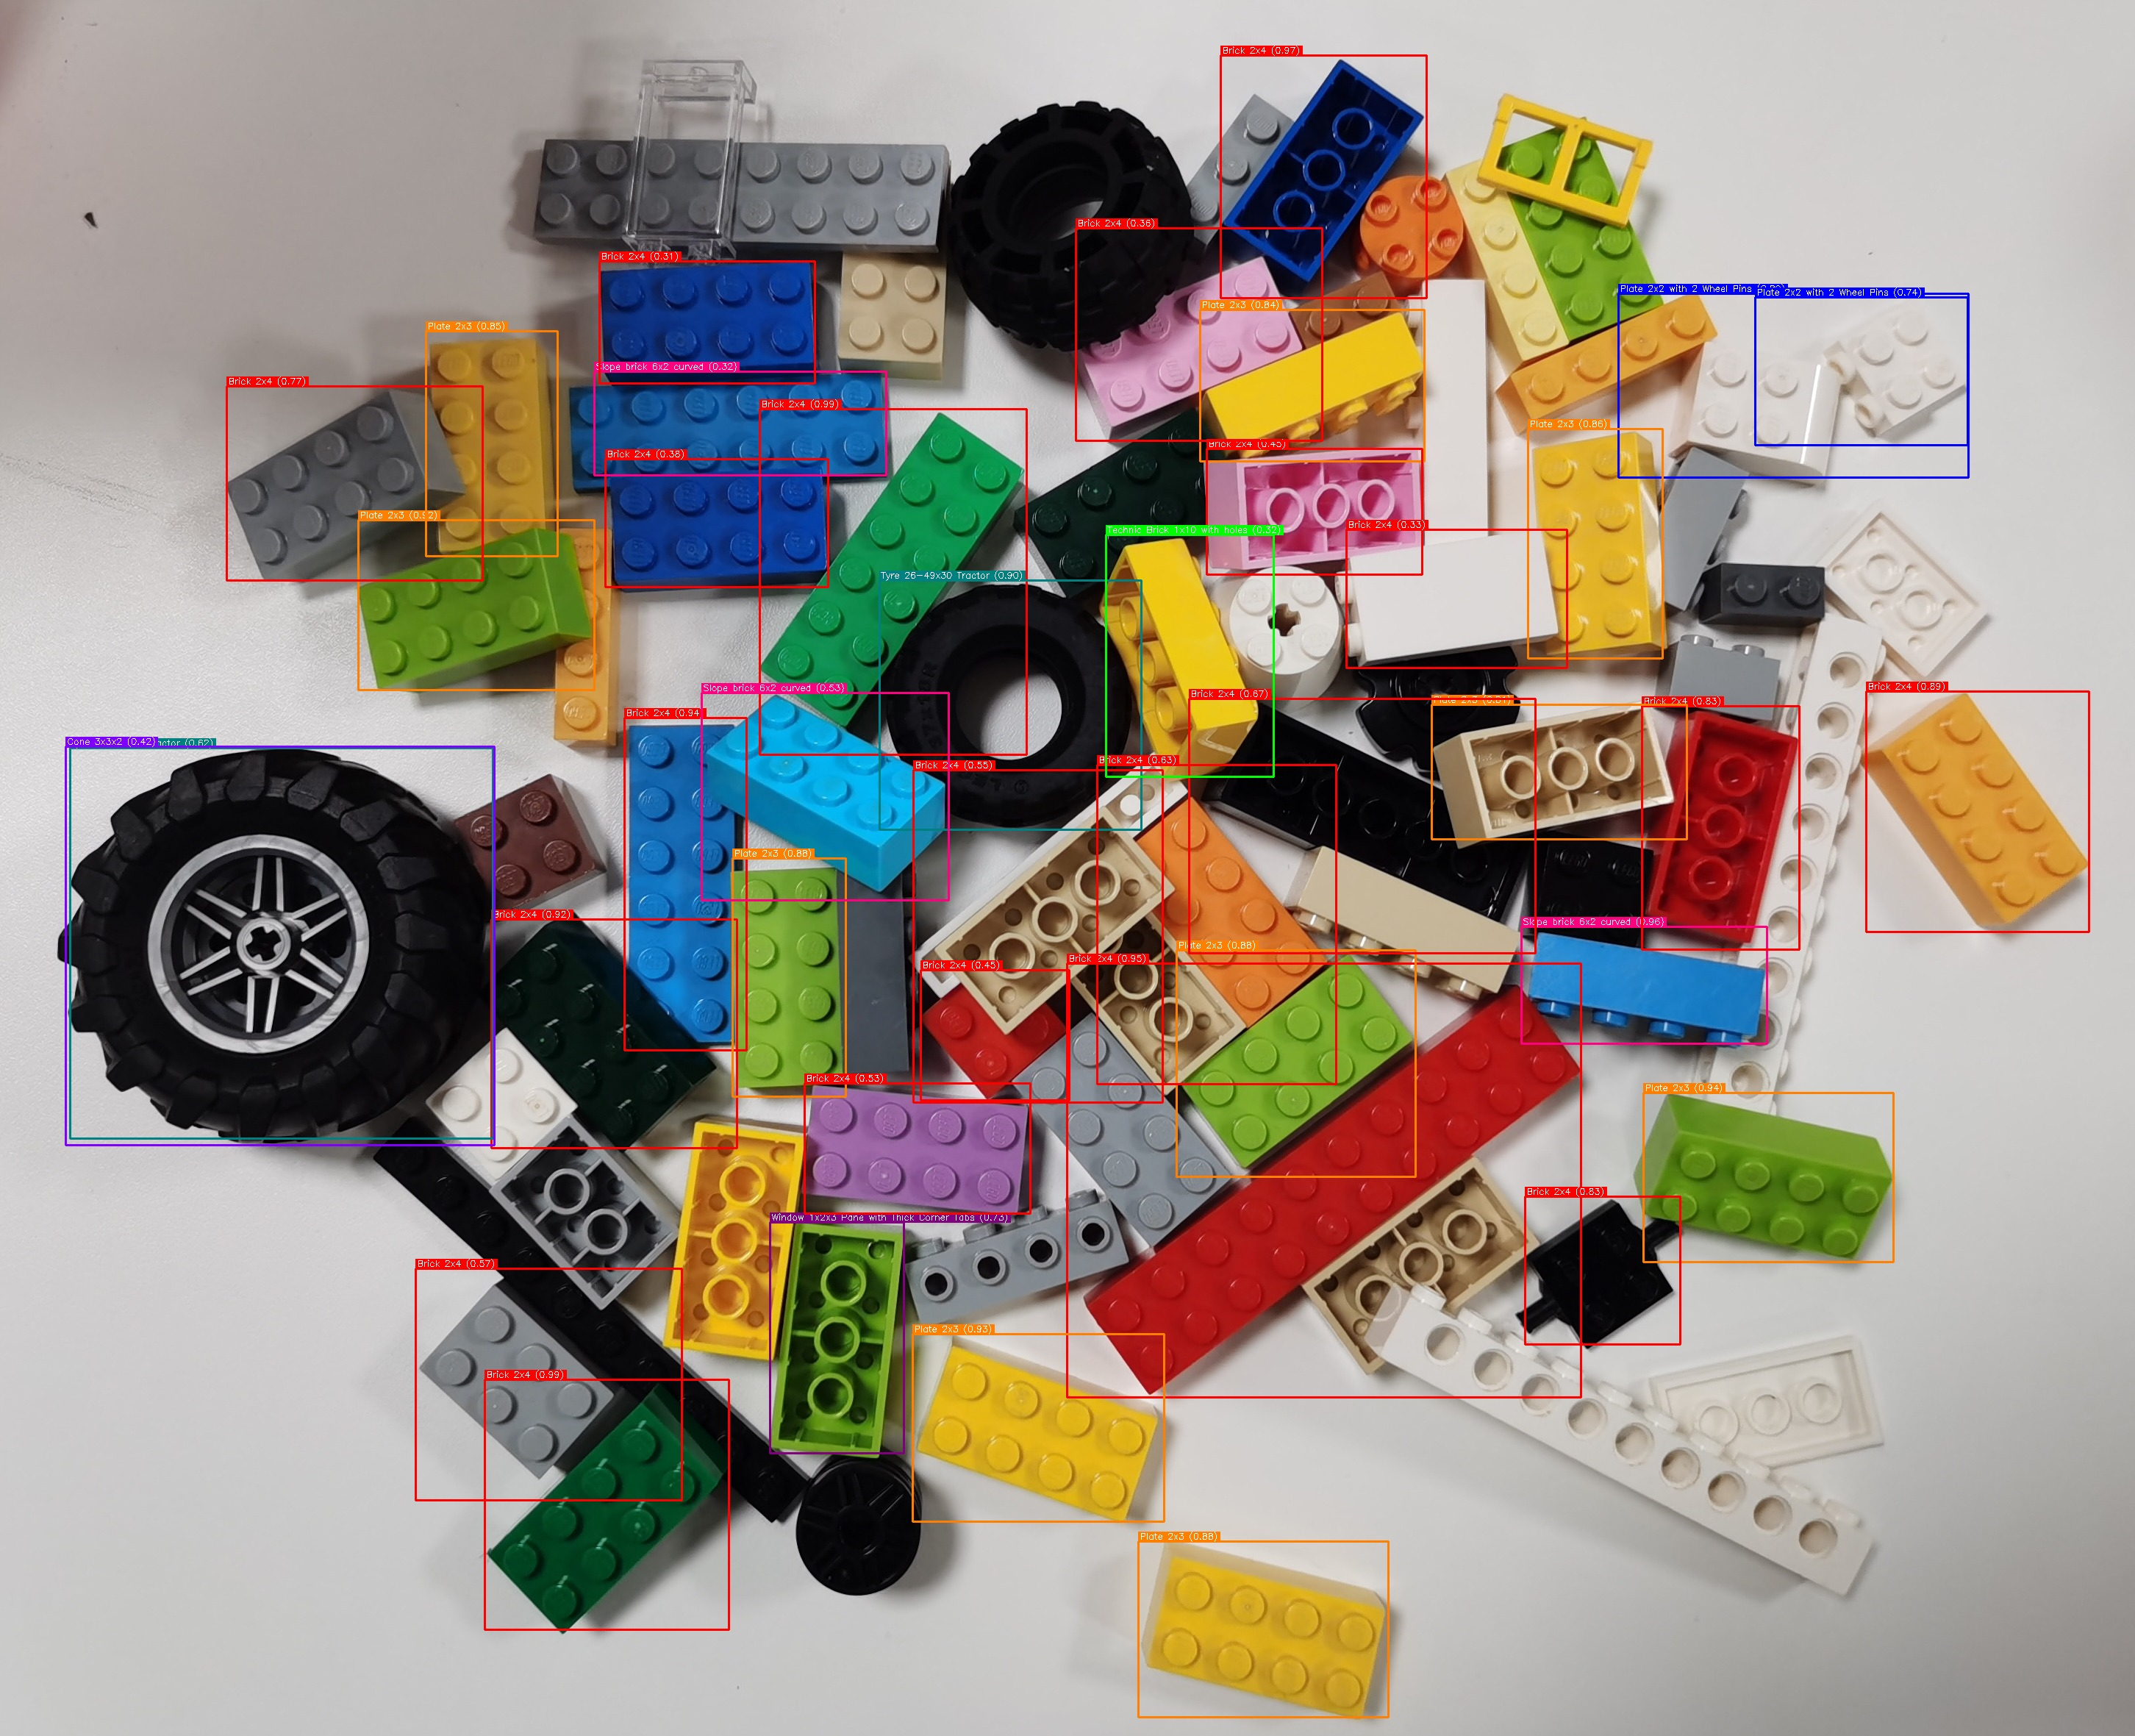
\includegraphics[width=\textwidth]{figures/detect_hard.jpg}
    \caption{困难难度代表（图 10）。检出 41 个零件，8 个类别，为全部图像中检出数最多。尽管存在一定遮挡，模型仍能识别大部分零件。}
    \label{fig:det_hard}
\end{figure}

% ═══════════════════════════════════════════════════════════
\section{讨论}
% ═══════════════════════════════════════════════════════════

\subsection{性能分析}

\textbf{优点}：模型能够以较高置信度可靠地检测常见零件（Brick 2x4、Plate 2x3）。即便某些稀有零件（如轮胎、链轮）在训练数据中仅有一张模板图像，模型仍能在部分测试图像中检出它们。

\textbf{不足}：
\begin{itemize}
    \item \textbf{紧密拼接的零件}（见第 4.3 节）是主要的失败场景。
    \item \textbf{俯视角度下外观相似的零件}：Brick 和 Plate 在课程要求中已允许合并，但其他相似零件（如不同型号的轮毂、轮胎）仍可能被混淆。
    \item \textbf{训练数据不充分的类别}：仅有一张模板图像且只有一种颜色变体的零件，漏检率明显更高。
\end{itemize}

\subsection{合成训练数据的局限性}

\begin{table}[H]
    \centering
    \caption{合成数据的主要局限}
    \label{tab:limitations}
    \begin{tabular}{lp{10cm}}
        \toprule
        \textbf{局限} & \textbf{影响} \\
        \midrule
        领域差异 & 合成图像与真实照片在光照、阴影、表面纹理等方面存在差异。预处理流程部分弥合了这一差距，但仍有残余。 \\
        无紧密拼接 & 数据生成器在零件之间添加随机间距，从未模拟零件无缝卡合的场景。 \\
        颜色多样性不足 & 大多数模板图像仅有一种颜色变体，而测试图像中的零件颜色丰富多样。 \\
        遮挡模型简单 & 30\% 的随机重叠概率可能与困难级别图像中的真实遮挡模式不完全匹配。 \\
        \bottomrule
    \end{tabular}
\end{table}

\subsection{失败案例分析：图 2}

图 2 中相同颜色的积木紧密排列成规整的网格。模型仅检出 \textbf{2 个零件}（均为 Brick 2x4，置信度分别为 0.35 和 0.79），而图像中的实际零件数量远多于此。

\begin{figure}[H]
    \centering
    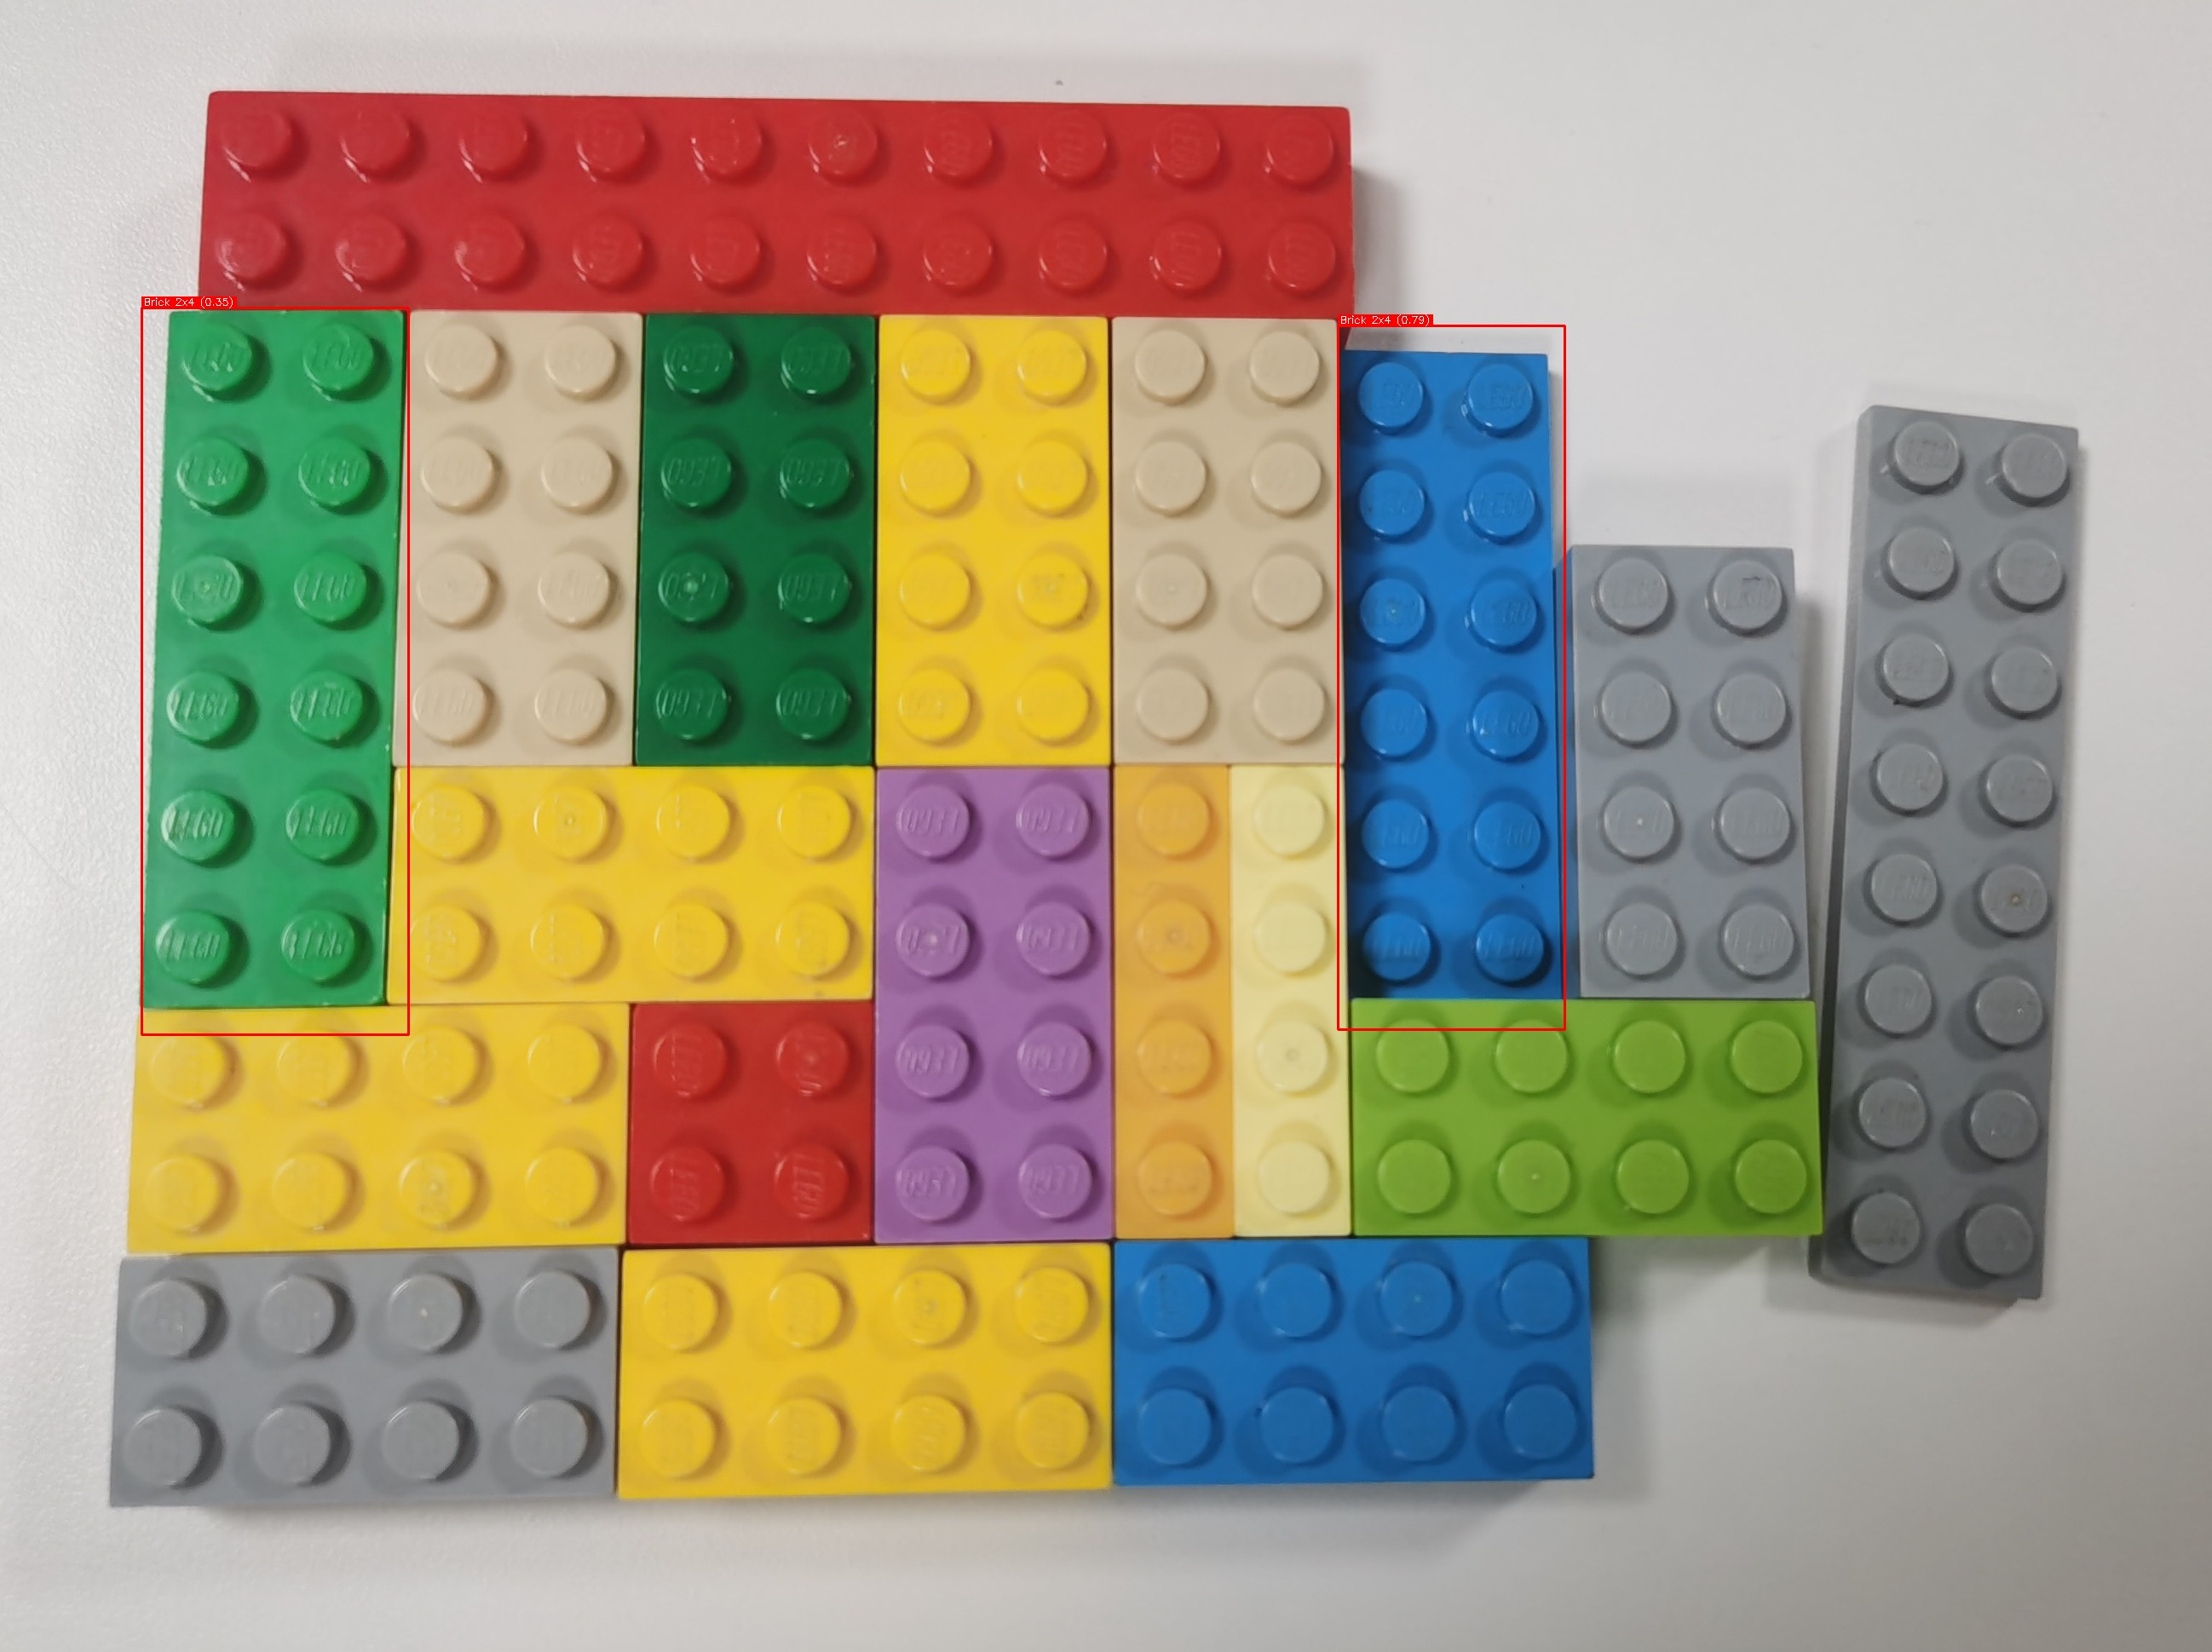
\includegraphics[width=0.85\textwidth]{figures/detect_failure.jpg}
    \caption{失败案例（图 2）。仅检出 2 个 Brick 2x4，大量紧密拼接的同色砖块被漏检。注意图中仅有两个绿色检测框覆盖了部分区域，其余紧密排列的砖块完全未被识别。}
    \label{fig:det_failure}
\end{figure}

\textbf{根本原因}：同色且紧密卡合的相邻积木从俯视角度呈现为一个连续的矩形区域。相邻零件之间的接缝线在原图分辨率（$2596\times1939$）下仅有 1--2 像素宽。当图像被缩放到 $640\times640$ 送入 YOLO 推理时，这些接缝被压缩到亚像素级别，完全消失。

这是合成数据策略的一个系统性盲区：训练数据生成器\emph{从未创建}过同色零件紧密相邻排布的训练样本。模型因此无法学会将发丝般的接缝作为边界线索。

为应对这一问题，我们探索了一种基于高斯差分滤波（DoG）的传统计算机视觉方法，用于检测亚像素级别的细缝线，但该方案目前仅作为辅助分析工具。

% ═══════════════════════════════════════════════════════════
\section{结论与展望}
% ═══════════════════════════════════════════════════════════

本项目实现了一套完整的自动化乐高零件计数流程。通过从模板图像生成合成训练数据并微调 YOLOv8 检测模型，系统在无需人工标注的条件下取得了可观的检测效果：从 10 张测试图像中检出 \textbf{241 个零件，覆盖 16/18 个类别}。

\textbf{主要发现}：

\begin{enumerate}
    \item 合成训练数据是该领域的有效替代方案，在合成验证集上达到 mAP@50 = 0.899。
    \item 主要失败模式为同色紧密拼接零件，其边界在推理分辨率下不可见。这直接导致了图 2 近乎完全的检测失败。
    \item 仅有一张模板图像的零件类别检测可靠度较低，增加模板多样性有望提升效果。
\end{enumerate}

\textbf{未来工作方向}：

\begin{itemize}
    \item 将传统计算机视觉的细缝检测（基于 DoG）与深度学习结果进行融合。
    \item 改进合成数据生成器，使其能够建模零件无缝相邻排列的场景。
    \item 收集更多颜色和角度的模板图像，提升训练数据多样性。
    \item 探索实例分割模型（YOLOv8-seg），以更好地分离相互接触的零件。
    \item 结合合成数据与少量真实标注数据进行半监督或小样本微调。
\end{itemize}

\end{document}
